% !TeX spellcheck = en_GB

\PassOptionsToPackage{implicit=true}{hyperref}

\documentclass[10pt, aspectratio=1610, compress, protectframetitle, handout]{beamer}
\usefonttheme{professionalfonts}
\setbeamertemplate{blocks}[rounded][shadow=true]

\usepackage[normalem]{ulem}
\usepackage[T1]{fontenc}
\usepackage{graphicx}
\usepackage{booktabs}
\usepackage{wrapfig}
\usepackage{float}
\usepackage{datetime}
\usepackage{textpos}
\usepackage{xcolor}
\usepackage{bm}
\usepackage[ruled,vlined]{algorithm2e}
\usepackage{mathtools}
\usepackage[autostyle]{csquotes}
\usepackage[export]{adjustbox}

\MakeOuterQuote{"}

\usepackage{appendixnumberbeamer}
\usepackage[british]{babel}
\usepackage{wrapfig}
\usepackage{emoji}

\usetheme[titleformat=regular, sectionpage=progressbar, subsectionpage=none, numbering=fraction, progressbar=frametitle, block=fill]{metropolis}
\setmonofont{FiraMono-Regular.otf}

\graphicspath{{img/}}

\definecolor{MetroLinks}{RGB}{96, 76, 56}
\definecolor{MetroCite}{RGB}{35, 55, 59}
\definecolor{MetroUrl}{RGB}{20, 176, 61}

\hypersetup{
    colorlinks,
    linkcolor=MetroLinks,
    citecolor=MetroCite,
    urlcolor=MetroUrl,
}

\DeclareMathOperator*{\argmax}{arg\,max}
\DeclareMathOperator*{\argmin}{arg\,min}
\DeclareMathOperator*{\kldiv}{\text{KL}}
\newcommand{\cardof}[1]{|#1|}
\newcommand{\condon}{|}
\newcommand{\ddiff}[1]{\mathop{d#1}}
\newcommand{\dimof}[1]{\text{dim}(#1)}
\newcommand{\dpart}[1]{\mathop{\partial#1}}
\newcommand{\fullstop}{\text{ .}}
\newcommand{\mat}[1]{\bm{#1}}
\newcommand{\netw}[1]{\mathcal{#1}}
\newcommand{\normof}[1]{||#1||}
\newcommand{\suchthat}{\textit{s.t.\ }}
\newcommand{\etc}{\textit{etc.\ }}
\newcommand{\wlogg}{\textit{w.l.o.g.\ }}
\newcommand{\wrt}{\textit{w.r.t.\ }}
\renewcommand{\vec}[1]{\bm{#1}}
\newcommand{\carso}{\texttt{CARSO}\ }

% Change Colors/Width of Progress Bars
\makeatletter
\setlength{\metropolis@progressonsectionpage@linewidth}{3pt}
\makeatother

% Quoting tools
\let\oldquote\quote
\let\endoldquote\endquote
\renewenvironment{quote}[2][]
{\if\relax\detokenize{#1}\relax
    \def\quoteauthor{#2}%
    \else
    \def\quoteauthor{#2~---~#1}%
    \fi
    \oldquote}
{\par\nobreak\smallskip\hfill(\quoteauthor)%
    \endoldquote\addvspace{\bigskipamount}}


\title{\textsc{\texttt{C}ounter\texttt{A}dversarial \texttt{R}ecall of \texttt{S}ynthetic \texttt{O}bservations}}
\subtitle{A \textit{neuro-inspired} approach to foil gradient-based adversarial attacks}
\author{Emanuele \textsc{Ballarin}\inst{$\dagger$}}
\institute[]{
    \inst{$\dagger$} \scshape{\texttt{AICPS} $\in$ Dept. of Mathematics $\subseteq$ Univ. of Trieste} |
    \inst{$\ddagger$} \scshape{\texttt{AREA} Science Park}
}

\addtobeamertemplate{frametitle}{}{%
    \begin{textblock*}{100mm}(0.8\textwidth,-0.94cm)
        \hspace{10px}
        
\includegraphics[valign=c, height=0.4cm]{logo_adsai_bw_scaled}
        \hspace{3px}
        
\includegraphics[valign=c, height=0.4cm]{logo_dssc_white}
        \hspace{2px}
        
\includegraphics[valign=c, height=0.45cm]{logo_units_white}
\end{textblock*}}

\AtBeginSection[]
{
    \begin{frame}
        \vspace*{30px}
        \frametitle{\protect{\emoji{round-pushpin}} \textit{We are here}}
        \tableofcontents[currentsection]
    \end{frame}
}

\begin{document}
    % !TeX spellcheck = en_GB

\setbeamertemplate{title page}{
    \begin{minipage}[b][\paperheight]{\textwidth}
        \ifx\inserttitlegraphic\@empty\else\usebeamertemplate*{title graphic}\fi
        \vfill
        \ifx\inserttitle\@empty\else\usebeamertemplate*{title}\fi
        \ifx\insertsubtitle\@empty\else\usebeamertemplate*{subtitle}\fi
        \usebeamertemplate*{title separator}
        \vspace*{4px}
        \begin{minipage}[]{0.5\textwidth}
            \ifx\beamer@shortauthor\@empty\else\usebeamertemplate*{author}\fi
            \vspace*{1.8em}
        \end{minipage}
        \begin{minipage}[]{0.5\textwidth}
            \raggedleft
            {\small Supervised by: Prof. Luca \textsc{Bortolussi}{${}^\dagger$} \par}
            \vspace*{0.2em}
            {\small CoSupervised by: Dr. Alessio \textsc{Ansuini }{${}^\ddagger$}}
        \end{minipage}
        \vspace*{7px}
        \center\small Graduation session: M.Sc. in \textit{Data Science and Scientific Computing}
        \center\ifx\insertdate\@empty\else\usebeamertemplate*{date}\fi
        \vspace*{14px}
        \raggedright\ifx\insertinstitute\@empty\else\usebeamertemplate*{institute}\fi
        \vspace*{15px}
    \end{minipage}
}

\frame{\titlepage}

    % !TeX spellcheck = en_GB

\begin{frame}{\protect{\emoji{scroll}} \textit{A plan for the next $\sim$$0.5\text{h}$}}

    \begin{center}
    \underline{An \textit{elevator pitch}}
    \end{center}

    \texttt{CARSO} (\textit{CounterAdversarial Recall of Synthetic Observations}) is a \alert{novel} \textit{deep learning} architecture and training/inference methodology for the improvement of \alert{\textit{adversarial robustness}} in \textit{deep artificial neural networks}.

    \begin{itemize}
        \item Loosely inspired by high-level \textit{neurocognitive} mechanisms;
        \item Targeted against \textit{\alert{gradient}-based}, \textit{white-box} attacks;
        \item Significant, promising results so far; comprehensive testing still in early stages.
    \end{itemize}

\end{frame}
    % !TeX spellcheck = en_GB

\section{\protect{\emoji{chipmunk}} \textit{Deep Learning} in a nutshell}{

    \begin{frame}{\protect{\emoji{chipmunk}} \textit{Deep Learning}: a definition}

        \begin{block}{\textit{Deep Learning}}
            \textit{Deep Learning} is (probabilistic) \alert{\textit{machine learning}} with \textit{deep artificial \alert{neural networks}, operating in (strongly) \alert{overparametrised} regime.}
        \end{block}
        \begin{center}
            OK, but what does it mean?
        \end{center}

    \end{frame}

    \begin{frame}{\protect{\emoji{chipmunk}} \textit{Deep Learning} $\subseteq$  \textit{Machine Learning}}

        \begin{block}{\textit{Machine Learning}}

            \begin{quote}{\textsc{T. Mitchell}, \textit{attributed} -- 1997}
                \hfill\break
                A computer program is said to learn from experience E w.r.t. to some class of tasks
                T and performance measure P, if its performance at tasks in T, as measured by P,
                improves with experience E.
            \end{quote}
        \end{block}

        Allowing effective decoupling of:
        \begin{itemize}
            \item \alert{\textit{model}} (in our case: \textit{artificial neural networks})
            \item \alert{\textit{learning algorithm}} (in our case: \textit{loss} function minimisation; approximate, iterative, gradient based\footnote{Not strictly necessary, though})
        \end{itemize}
    \end{frame}
    \setcounter{footnote}{0}

    \begin{frame}{\protect{\emoji{chipmunk}} An intermezzo: \textit{Supervised Classification}}

        \underline{Focus scenario for today: \textit{supervised learning}}.
        \hfill\break

        \textit{Input} space: $\mathbb{I} \sim \mathbb{R}^{d}$ -- \textit{What} needs to be classified, or their embedding;\\
        \textit{Output} space: $\mathbb{O}$ -- Set of classes to \alert{partition} $\mathbb{I}$ in (or \textit{e.g.} \textit{logits}, \etc).\\
        \hfill\break
        \textit{Training set}: $\{\mathbb{I}\times\mathbb{O}\} \supseteq \mathbb{T} = \{(\vec{x}_1, \xi_1), (\vec{x}_2, \xi_2), \ \dots,\ (\vec{x}_n, \xi_n)\}$ -- Known examples;
        \hfill\break
        A classifier $\mathcal{N}_{\vec{\theta}, \vec{h}}: \ \mathbb{I} \rightarrow \mathbb{O}$ dependent from  \alert{parameters}\footnote{And statistics of the data; \textit{computed} rather than \textit{learned} optimisation-wise} ($\vec{\theta}$) and \alert{hyperparameters} ($\vec{h}$);\\
        A \alert{\textit{loss function}}: $\mathcal{L} = \mathcal{L}(\mathcal{N}_{\vec{\theta}, \vec{h}}, \mathbb{T})$ encoding the \textit{goodness} of the model on $\mathbb{T}$.
        \hfill\break

        \begin{block}{Goal of \textit{training}}

            Find optimal $\vec{\theta}$, \textit{i.e.} $\vec{\theta^{\star}} \coloneq \argmin_{\vec{\theta}}(\mathcal{L}(\mathbb{T} | \vec{\theta}, \mathcal{N}_{\vec{\theta},\vec{h}}))$
        \end{block}

    \end{frame}
    \setcounter{footnote}{0}

    \begin{frame}{\protect{\emoji{chipmunk}} The model: from \textit{neurons} to \textit{neural networks}}

        Preliminarily, we consider the \textit{vector-scalar} map $\netw{N}_{\textit{1n}}\colon \mathbb{R}^{d}\rightarrow\mathbb{R}$ (\textit{McCulloch-Pitts neuron}): an \alert{affine} transformation followed by a \alert{nonlinear} application, \textit{i.e.:}
        $$ y = \netw{N}_{\textit{1n}}(\vec{x}) = \mathcal{A}(b + \vec{w}\cdot\vec{x}) $$
        with learnable parameters $\vec{\theta} = (\vec{w}, b)$.

        For a \textit{vector-vector} map $\netw{N}_{\textit{1n}}\colon \mathbb{R}^{d}\rightarrow\mathbb{R}^{m}$, we operate element-wise \wrt the output, defining a \textit{neuron layer}, \textit{i.e.}:
        $$ \vec{y} = L(\vec{x}) = \mathcal{A}(\vec{b} + \mat{W}\vec{x}) \fullstop $$

        Such transformations can be composed, for (\alert{arbitrary}\footnote{Usually in the \textit{function space density} sense -- more generally \textit{PAC-ly} -- given \textit{width/depth} and growing the other.}) increased expressive power, in a \textit{fully connected}, \textit{feedforward} artificial neural network:
        $$ \vec{y} = \netw{N}(\vec{x}) = L_n(L_{n-1}(\dots L_2(L_1(\vec{x})))) \fullstop$$

    \end{frame}
    \setcounter{footnote}{0}

    \begin{frame}{\protect{\emoji{chipmunk}}Learning $\vec{\theta^{\star}}$: \textit{SGD \& friends}}

        We are left with an \alert{optimisation} problem in the (potentially \textit{very high-dimensional}) space of $\vec{\theta}$, that is generally \alert{intractable}. We resort to an \textit{iterative}, \textit{first-order}, approximate optimisation scheme. \textit{E.g.} (\textit{gradient descent with momentum}):

        $$ \vec{\theta^{\prime}} \leftarrow \vec{\theta} - \lambda\alert{\vec{g_i}} + \alert{\mu\vec{m}}$$
        $$ \vec{m^{\prime}} \leftarrow \vec{\theta^{\prime}} - \vec{\theta}\fullstop$$

        Usually, \textit{minibatch-aggregation}\footnote{Often, \textit{gradient averaging} over disjoint subsets of training data} and further \alert{regularisation} (\textit{e.g.} penalisation at \textit{loss} or \textit{weight} level\footnote{Source of the \textit{proper} $L_2$ \textit{vs.} \textit{proper weight decay} divergence.}) is employed.
    \end{frame}

    \begin{frame}{\protect{\emoji{chipmunk}} That's \textit{not} all, folks!}

        That was just a \textit{sneak peek}, and there is much much more...
        \begin{itemize}
            \item Different architectural \alert{\textit{inductive biases}} (\textit{e.g. convolutional-, graph- NNs});
            \item More advanced optimisers (\textit{e.g. EMA-based -- à la Adam, nested, $>1^{\textit{st}}$-order});
            \item Other regularisation strategies, \textit{convergence/generalisation} aids (\textit{i.e.} \textit{BatchNorm}, \textit{dropout});
            \item Learning rate scheduling and hyperparameter tuning;
            \item \alert{Efficient} gradient computation (\textit{e.g.} via \textit{BackProp});
            \item \textit{AutoDiff} internals, \etc\dots
        \end{itemize}
    \hfill\break
    We showed just a \textit{bare minimum} to allow what follows (\textit{but if time allows...}).

    \end{frame}

    \begin{frame}{\protect{\emoji{thinking-face}} \textit{Is everything clear?}}

    \textit{Fast-forwarding} to-date, \textit{deep learning} is a remarkably powerful and mature paradigm, able to reach (super)human-level performance in selected \textit{regression}, \textit{classification}, data \textit{generation} and \textit{control} tasks.

    \center 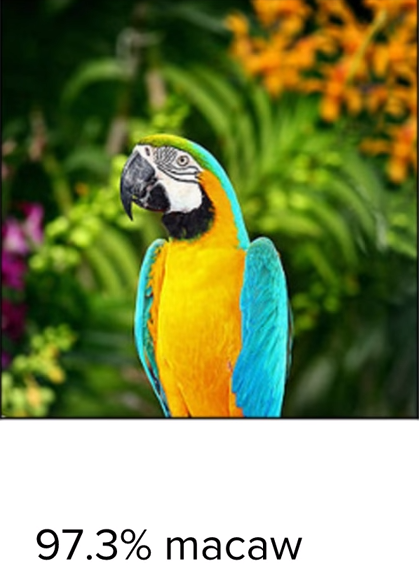
\includegraphics[height=0.35\linewidth]{macaw_macaw.png}
    \end{frame}

    \begin{frame}{\protect{\emoji{thinking-face}} \textit{Maybe not.}}

    \center 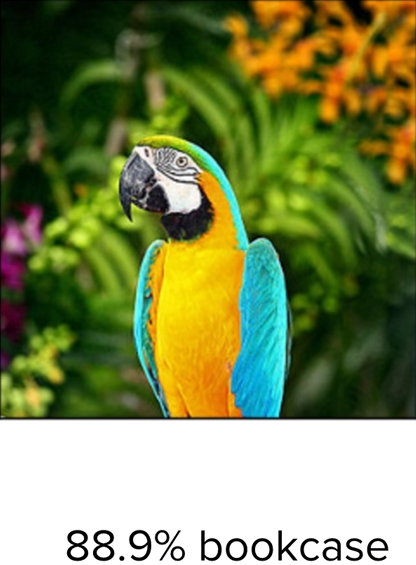
\includegraphics[height=0.35\linewidth]{macaw_bookcase.png}

    \hspace*{14px}\textit{(P. Perdikaris, 2018)}
    \end{frame}
    \setcounter{footnote}{0}
}
    % !TeX spellcheck = en_GB

\section{\protect{\emoji{thinking-face}} The problem of \textit{adversarial robustness}}{

    \begin{frame}{\protect{\emoji{thinking-face}} \textit{Adversarial inputs and attacks}}
        The last shown picture is an example of
        \hfill\break
        \begin{block}{\textit{Adversarial Input}}
            An \textit{input} is said to be \textit{adversarial} to a machine learning system if it alters its \alert{reasonably} expected behaviour\footnote{Usually from the \textit{P.o.V.} of the user(s).}. Also called \textit{adversarial attack}, stressing the intentional\footnote{Which is not a strict requirement, though!} crafting of it.
        \end{block}

    In the specific case of a classifier: produce a \textit{misclassification}.
    \end{frame}


    \begin{frame}{\protect{\emoji{thinking-face}} Why studying \textit{adversarial robustness}?}

        We live in times where a growing portion of even \textit{high-stakes} \alert{decisions} is \alert{delegated} to autonomous systems (\textit{e.g.} \textit{HR} selection, insurance, health, fraud detection, \etc\dots).\\$\rightarrow$ The example of \textit{Lemonade} \protect{\emoji{lemon}}

        \underline{Purely \textit{technical} reasons}
        \begin{itemize}
            \item Harden \textit{ML/DL} systems against \alert{misuse} and \textit{input-tampering};
            \item Assess (and \textit{\alert{patch}!}) behaviour where it the most fragile.
        \end{itemize}

        \underline{\textit{Legal / ethical / social} reasons}
        \begin{itemize}
            \item To ensure \alert{compliance} with regulatory frameworks or coordinated initiatives thereof;
            \item Increase understanding, transparency, and societal \alert{trust}.
        \end{itemize}

        \underline{Broader-reaching goals}
        \begin{itemize}
            \item Use \textit{robustness} as a lens through which to study \textit{\alert{neurocognitive} phenomena}.
        \end{itemize}
    \end{frame}

    \begin{frame}{\protect{\emoji{thinking-face}} Where things \textit{go awry}: the \textit{Manifold Hypothesis} (I)}

        An intuitive geometrical characterisation of \textit{adversarial attacks} can be done in the light of the

        \begin{block}{\textit{\alert{Manifold} Hypothesis}}
            \textit{Natural} high-dimensionally-coded data lie on (a) \alert{low-dimensional} manifold(s), immersed within the high-dimensional allowed \textit{code space}.
        \end{block}

    This partitions the \textit{code space} in \textit{four} regions:
    \begin{enumerate}
        \item Expected behaviour region (\textit{on-manifold});
        \item Cross-boundary adversarial region (\textit{\alert{on}-manifold});
        \item \textit{Natural} non-applicability region (\textit{\alert{along} manifold});
        \item "Negative space" adversarial region (\textit{\alert{off}-manifold}).
    \end{enumerate}

    \end{frame}

    \begin{frame}{\protect{\emoji{thinking-face}} Where things \textit{go awry}: the \textit{Manifold Hypothesis} (II)}
        \begin{center}
            "A picture is worth thousand words". (\textit{Here's $2\times10^3$!})
        \end{center}

        \begin{minipage}[c]{0.49\textwidth}
            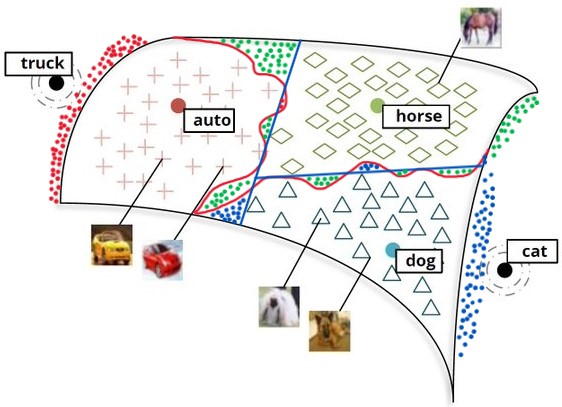
\includegraphics[width=1\textwidth, height=1\textheight, keepaspectratio]{manifold-hyp}
        \end{minipage}
        \begin{minipage}[c]{0.49\textwidth}
            \vspace{0pt}
            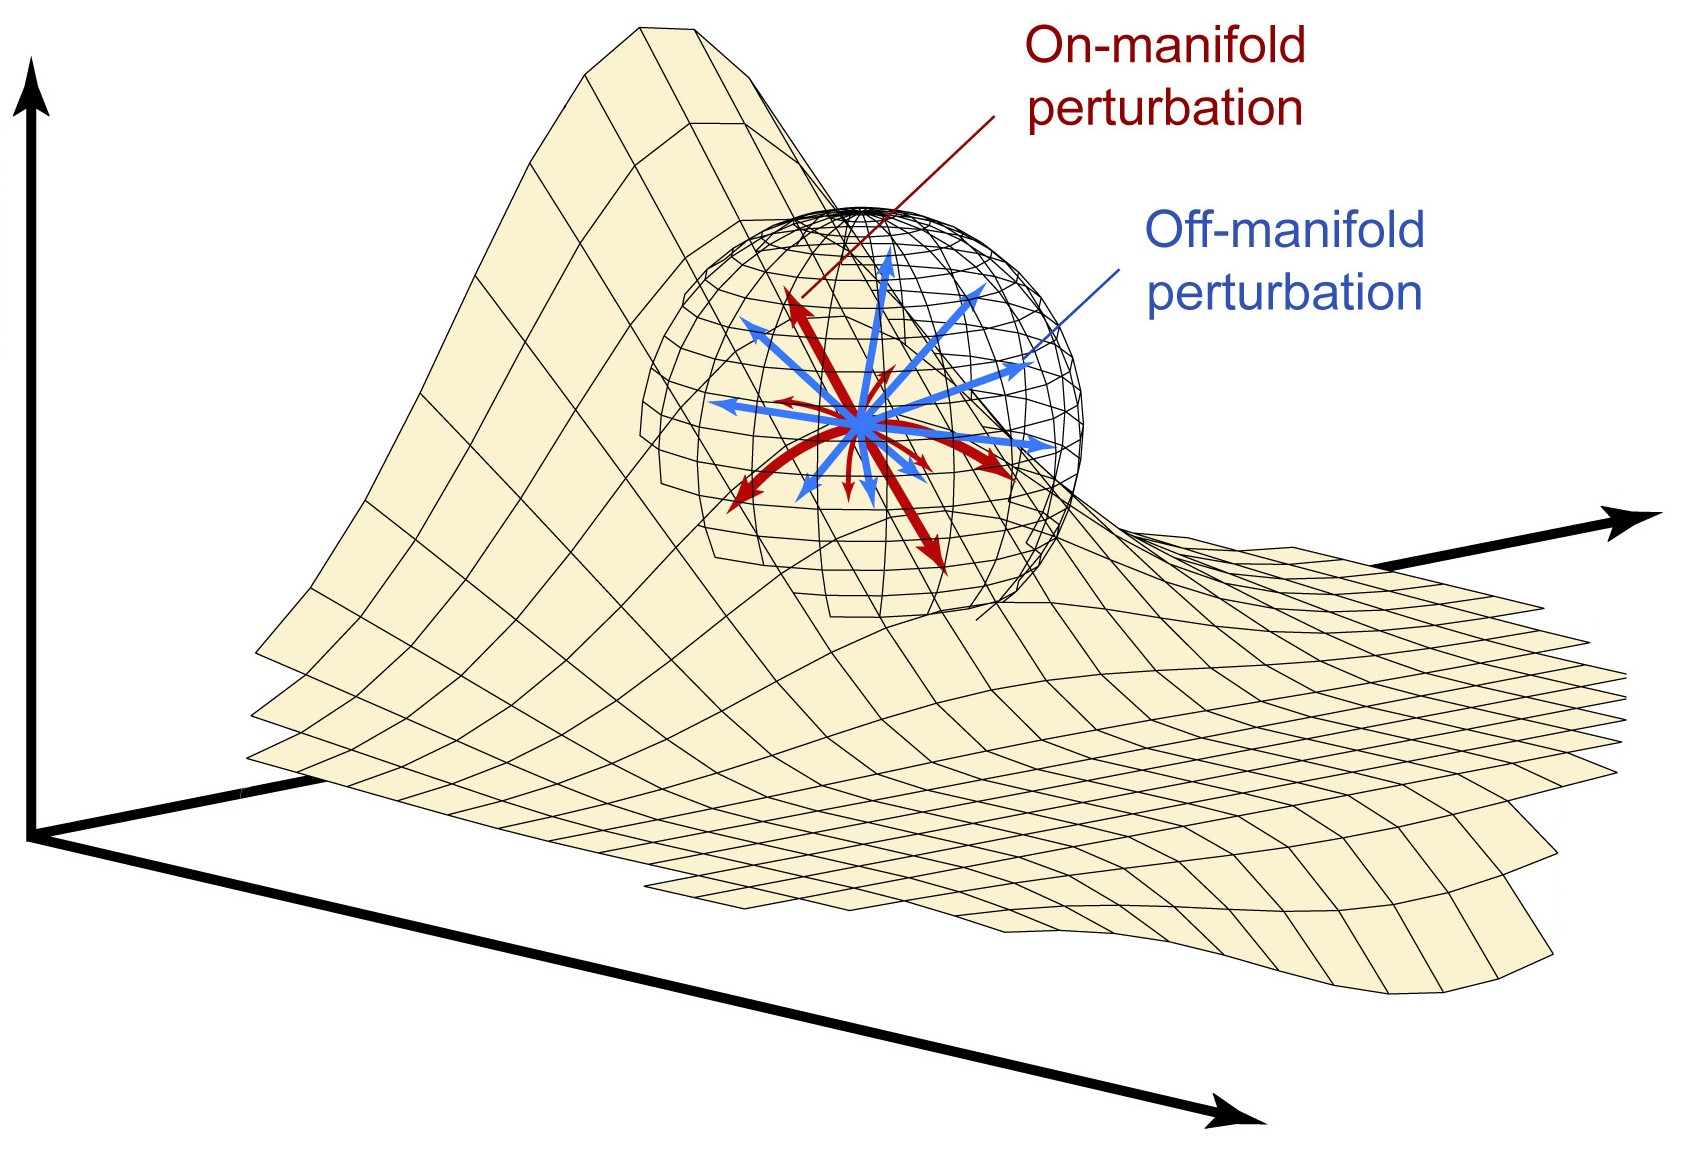
\includegraphics[width=1\textwidth, height=1\textheight, keepaspectratio]{manifold_ball_perturbations}
        \end{minipage}

    \end{frame}

    \begin{frame}{\protect{\emoji{thinking-face}} A (more) precise definition of \textit{robustness}}

        We can always reformulate the problem of \textit{adversarial inputs} as one of \textit{\alert{adversarial perturbations}}, \textit{i.e.}
        $$ \vec{x}_{\text{adversarial}} \coloneq  \vec{x}_{\text{legitimate}} + \alert{\vec{p}}$$

        leading to the following

        \begin{block}{Definition: \textit{\alert{$\epsilon$}-perturbative adversarial attack against classifier $\netw{N}$ in $x_0 \in \mathbb{I}$, \wrt $\normof{\cdot}$}}
            Any $\vec{x^{\star}} \coloneq \vec{x_0} + \vec{p} \text{ | } \netw{N}(\vec{x^{\star}}) \neq \netw{N}(\vec{x_0})$ and $\normof{\vec{p}} < \epsilon$
        \end{block}

    \underline{Minimal systematics}:
    \begin{itemize}
        \item \textit{black box} vs. \textit{\alert{white box}};
        \item \textit{targeted} vs. \textit{\alert{untargeted}}.
    \end{itemize}

    Needless to say: \textit{the world is not so simple; however...}
    \end{frame}

    \begin{frame}{\protect{\emoji{thinking-face}} \textit{How it's done}: attacks}

        \underline{\textit{White-box} scenario}
        \begin{itemize}
            \item Direct, \alert{gradient}-based (\textit{e.g.} \texttt{FGSM} \& derived);
            \item Iterative, \alert{gradient}-based (\textit{e.g.} \texttt{PGD}, \texttt{DeepFool});
            \item Specific response-elicitation methods (\textit{e.g.} \textit{k-pixel} attack, \textit{noisy \texttt{FGSM}}).
        \end{itemize}

        \underline{\textit{Black-box} scenario}
        \begin{itemize}
            \item \textit{Gradient-free} optimisation schemes;
            \item Direct-sampling \textit{generative} methods (\textit{e.g.} \texttt{AdvGAN(++)});
            \item \textit{White-box} methods towards \alert{surrogate} models (\textit{e.g.} \textit{Tramèr ensemble}).
        \end{itemize}

        \begin{block}{Definition: \textit{Universal Attack} (scheme)}
            A scheme for generating adversarial attacks able to reach \alert{any} point within the (chosen norm-induced) ball of radius $\epsilon$ ($\forall \epsilon$) centred in any \textit{legitimate} input point. Related: \textit{information \alert{optimal} attack}.
        \end{block}
    \end{frame}

    \begin{frame}{\protect{\emoji{thinking-face}} \textit{How it's done}: defences}

        That of \textit{adversarial robustness} research is a typical open, \textit{ladder-and-fence} scenario...\\
        With an even greater variability in defences:
        \begin{itemize}
            \item \textit{Adversarial training}: \alert{augment} $\mathbb{T}$ with correctly-labelled adversarial inputs (\textit{e.g.} \texttt{IAT});
            \item Adversarial detection: \alert{identify and handle} anomalous inputs (\textit{e.g.} \textit{\texttt{GAN}-discriminator anomaly detection});
            \item Adversarial purification: \alert{recover} \textit{clean} inputs from perturbed ones (\textit{e.g.} \texttt{PuVAE}, \texttt{DefenseGAN}, \textit{diffusion-based purification});
            \item \alert{Inference}-time defences: \textit{e.g.} \textit{filter} based, \textit{test-time augmentation} based, \etc;
            \item Robustly-\alert{structured} learning (\textit{e.g.} \textit{Parseval Networks});
            \item Paradigmatic shifts (\textit{e.g.} \textit{Bayesian} NNs).
        \end{itemize}
    \end{frame}

    \begin{frame}{\protect{\emoji{brain}} But, \textit{at the end of the day}...}

        No optimal, universal defence! Many \textit{case-by-case} results, many \textit{trade-offs}, practically no \textit{robust-by-design} applicable solution.
        \hfill\break

        \begin{block}{A remark}
            But... have \textit{\alert{you}} ever experienced an \textit{adversarial(-like) phenomenon?}
        \end{block}

    \end{frame}


}
    % !TeX spellcheck = en_GB

\section{\protect{\emoji{brain}} \textit{(relatively)} Robust neural systems: \textit{brains}}{

    \begin{frame}{\protect{\emoji{brain}} Adversarial attacks and the brain}

        \begin{center}
            \underline{Focus on vision}
        \end{center}

        It is safe to say that examples similar in form to \textit{adversarial attacks} for \textit{NNs} are \alert{yet to be discovered} for \textit{e.g.} human subjects.

        Some related phenomena, however, do \textit{probably} exist (within \textit{vision}):
        \begin{itemize}
            \item \alert{Retinal} response-elicitation (\textit{e.g. impossible colours}; incomplete evidence);
            \item \alert{Attention} retargeting via saliency shaping;
            \item Amygdala-mediated (\textit{\alert{semantic}}) attention retargeting;
            \item \alert{Fast}, \textit{adversarial} elicitation of the \alert{early} visual pathway (anecdotal).
        \end{itemize}

    ...and up to \textit{optical illusions}, with a stretch.
    \end{frame}

    \begin{frame}{\protect{\emoji{brain}} Recall, introspection... \textit{robust AI}?}

        Yet, \textit{brains} may be the \textit{only} practical realisation of a system with the \textit{robustness} properties we look for...

        \begin{block}{\protect{\emoji{light-bulb}} A guiding idea}
            Is it possible to loosely inform the development of \textit{robust} DL systems with (grossly simplified, idealised) descriptions of \alert{neurocognitive} phenomena?
        \end{block}

        Getting inspiration from the ideas of  \textit{\alert{recall} of acquired information}, and \textit{\alert{introspection}} as \textit{thought about thought}:
        \begin{itemize}
            \item Role of \textit{recall} as a \textit{\alert{comparison} tool} for newly acquired information;
            \item Role of \textit{recall} (and the aware \textit{anticipation} of it) in learning and \textit{\alert{gap-filling}} memories\\
            $\rightarrow$ \textit{Forward testing} phenomenon\\
            $\rightarrow$ \textit{Repeated testing} phenomenon
            \item \textit{Liminality} and hippocampal dynamics.
        \end{itemize}
    \end{frame}

    \begin{frame}{\protect{\emoji{brain}} An example from... poetry: \textit{recollection in tranquillity}}
        \centerline{
            \begin{minipage}[]{0.75\textwidth}
                \begin{quote}{\textsc{W. Wordsworth} -- \textit{I Wandered Lonely as a Cloud}}
                    \textelp{} I \alert{gazed}—and gazed—but little thought\\
                    What wealth the show to me had brought:\\
                    \mbox{}\\
                    For oft, when on my couch I lie\\
                    In vacant or in pensive mood,\\
                    They flash upon that \alert{inward eye} \textelp{}\\
                    $\textit{ }$
                \end{quote}
            \end{minipage}
        }
    \end{frame}

    \begin{frame}{\protect{\emoji{brain}} A crucial remark!}
        \begin{block}{\protect{\emoji{warning}} Beware!}
            The \textit{modelling} that follows has no claim of \textit{biological plausibility} whatsoever, at this stage! This would be \textit{added value}, though -- and in interesting research direction!
        \end{block}
    \end{frame}
}

    % !TeX spellcheck = en_GB

\section{\protect{\emoji{robot}} \texttt{CARSO}: an \textit{introspective artificial neural machine}}{

    \begin{frame}{\protect{\emoji{robot}} Core ideas and intuition (I)}

        Our synthetic \textit{thought process} (\underline{focus on \textit{classification}}):
        \begin{enumerate}
            \item All processing within a (non-stochastic) \textit{NN} is \alert{deterministic} at inference time;
            \item Different outputs from \textit{clean} and successfully \textit{perturbed} inputs must \textit{leave a \alert{different trace}} within the representation of a classifier;
            \item We can use such representation for \textit{adversarial detection}\\ $\rightarrow$ Unsatisfactory!
            \item \textit{And what about \alert{purification}}? We can inform a \textit{\alert{\texttt{cAE}}} with such representation;
        \end{enumerate}

    \begin{block}{Remark!}
    If the purified input is evaluated by the \textit{very same} classifier, the \textit{representation-as-hidden-layers} and the \textit{representation-as-\texttt{cAE}-input} induce \alert{competing} gradients for a \textit{gradient-based} adversary!
    \end{block}
    \end{frame}

    \begin{frame}{\protect{\emoji{robot}} Core ideas and intuition (II)}

    Our synthetic \textit{thought process} (cont.):
    \begin{enumerate}
        \setcounter{enumi}{4}
        \item At inference time, the \alert{representation is more than enough} to reconstruct the input;
        \item We can learn a \texttt{c\alert{V}AE} and sample from the specific purified-input space!
        \item Samples can be later classified and the outputs \alert{aggregated}.
    \end{enumerate}

    \begin{block}{Remark!}
    As a \textit{side effect}, this adds another layer of defence: a \textit{sampling-\alert{invariance}} for the adversary to overcome!
    \end{block}



    \end{frame}

    \begin{frame}{\protect{\emoji{robot}} Another intermezzo: \textit{Conditional Variational Autoencoders}}
        \begin{minipage}[]{0.5\textwidth}
    \vspace{0px}
    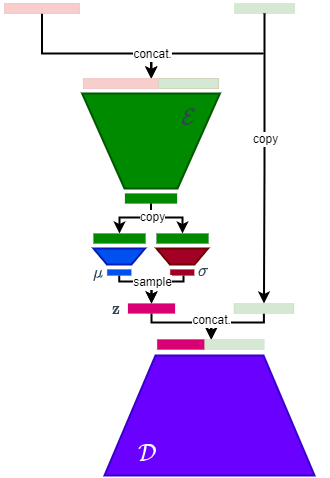
\includegraphics[width=0.91\textwidth, height=0.95\textheight, keepaspectratio]{cvae}
    \end{minipage}
    \begin{minipage}[]{0.45\textwidth}
        \vspace{0pt}
        \textit{Variational Autoencoders} are \textit{artificial neural architectures} able to \alert{sample} from probability densities in the form
        $$ \vec{x} \sim \vec{p}(\vec{\tilde{x}} \condon \phi_1, \dots, \phi_{s\in\mathbb{N}}) \fullstop$$

        They operate in \textit{standard} \alert{autoencoding} settings, with, additionally:
        \begin{itemize}
            \item Code-space sampling;
            \item The approximate \alert{reparametrisation}: $\vec{x} \approx \vec{\tilde{x}} = \netw{D}_{\vec{\theta_{\mathcal{D}}}}(\vec{c} \sim \vec{p}_{\text{latent}}(\vec{c}\condon \netw{E}_{\vec{\theta_{\mathcal{E}}}}(\vec{x})))$
            \item A \textit{loss} constraining the code distribution to a given \alert{structure}: $\mathcal{L}_{\texttt{VAE}} \coloneqq \mathcal{L}_{\text{AE}} + \kldiv(\vec{p}_{\text{latent}},\vec{p}_{\text{lobs}})$
        \end{itemize}

        \textit{Conditional \texttt{VAE}s} extend the sampling to \alert{conditional} distributions of the kind: $${\vec{\tilde{x}_{\text{r.v.}}} \sim \vec{p}(\vec{\tilde{x}_{\text{r.v.}}} \condon \vec{{x}_{\text{c.v.}}}, \phi_1, \dots, \phi_{s\in\mathbb{N}})}$$
    \end{minipage}
    \end{frame}

    \begin{frame}{\protect{\emoji{robot}} Training \texttt{CARSO}}
        \begin{minipage}[]{0.5\textwidth}
            \vspace{0px}
            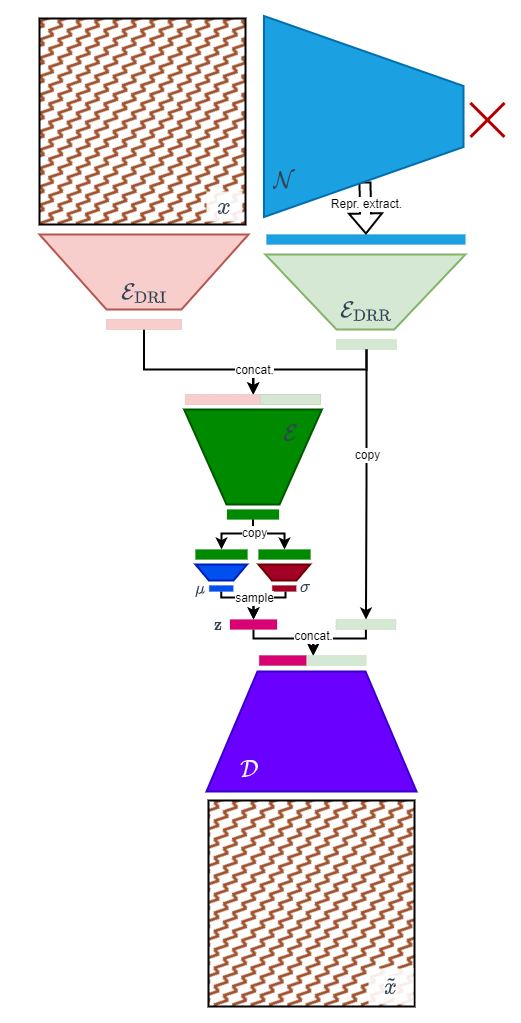
\includegraphics[width=0.91\textwidth, height=0.95\textheight, keepaspectratio]{traindiag}
        \end{minipage}
        \begin{minipage}[]{0.45\textwidth}
            \vspace{0pt}

            \begin{center}
                \underline{\textit{TL;DR:} Just a \textit{fancy \texttt{cVAE}}!}
            \end{center}

            Given an \textit{\alert{adversarially}-pretrained} classifier (for the problem of interest, and according to a given \textit{\alert{threat model}}):
            \hfill\break
            \begin{itemize}
                \item First \textit{classification pass} for representation \alert{extraction};
                \item Pre-encoding and \alert{rebalancing} of input \& representation;
                \item As in \texttt{cVAE}, aiming at \textit{\alert{purified} input} reconstruction from any input.
            \end{itemize}

        \begin{block}{Requirements}
            A dataset of \textit{clean/attacked} inputs to the classifier is needed (but \alert{no labels}!). Threat models may differ.
        \end{block}

        \end{minipage}
    \end{frame}

    \begin{frame}{\protect{\emoji{robot}} Inference with \texttt{CARSO}}
        \begin{minipage}[]{0.5\textwidth}
            \vspace{0px}
            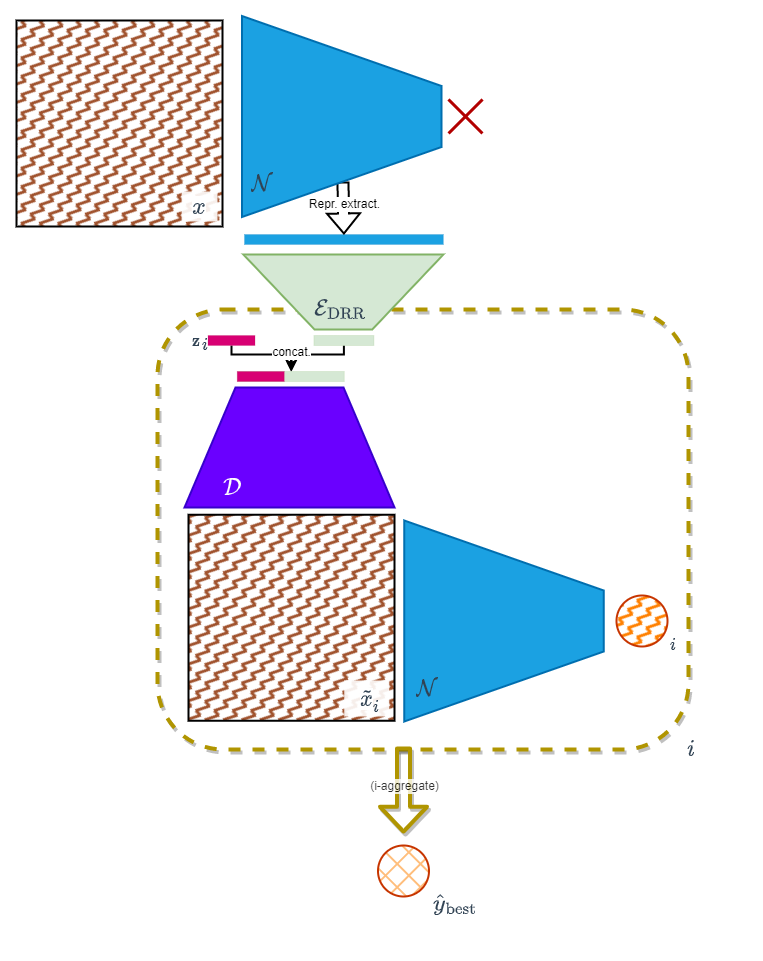
\includegraphics[width=0.95\textwidth, height=0.95\textheight, keepaspectratio]{inferdiag}
        \end{minipage}
        \begin{minipage}[]{0.45\textwidth}
    \vspace{0pt}

    \begin{center}
        \underline{\textit{TL;DR:} Condition, sample, classify, aggregate!}
    \end{center}

    Given the same \textit{adversarially-pretrained} classifier, the just-trained \textit{representation pre-compressor} and \textit{decoder}:
    \hfill\break
    \begin{itemize}
        \item First \textit{classification pass} for representation \alert{extraction};
        \item Representation \textit{pre-encoding};
        \item \alert{Repeated sampling} of \textit{candidate purified inputs};
        \item Second classification pass on such reconstructions, for \alert{actual classification};
        \item \alert{Aggregation} of results.
    \end{itemize}
    \end{minipage}
    \end{frame}

    \begin{frame}{\protect{\emoji{test-tube}} Will it work?}
        \centerline{
    \begin{minipage}[]{0.75\textwidth}
        \begin{quote}{\raggedleft\textsc{M. Budinich} -- \textit{"Introduction to the theory of NNs" course; final remarks before the exam}}
            The difference between a \textit{\alert{great idea}} and an \textit{idea that \alert{works}} is the part in which \alert{you} make it work.\\
            $\textit{ }$
        \end{quote}
    \end{minipage}
    }
    \end{frame}


}

    % !TeX spellcheck = en_GB

\section{\protect{\emoji{test-tube}} Experimental evaluation}{

    \setcounter{footnote}{0}

    \begin{frame}{\protect{\emoji{test-tube}} Experiment setup (I)}
    \underline{General goal}: \alert{accurate} -- but \textit{\alert{narrow}-scoped} -- investigation; beyond \textit{proof-of-concept}, not\\\hphantom{\underline{General goal}: }extensive. Focus on \alert{image classification} tasks.

    \underline{\textit{Foreseen attacks}}: whole-\alert{dataset} \texttt{FGSM} ($\normof{\cdot}_2$), \texttt{PGD} ($\normof{\cdot}_{\infty}$); various strengths\\\hphantom{\underline{\textit{Foreseen attacks}} } ($\epsilon=0.15$, $\epsilon=0.30$ \footnote{On normalised data, $\epsilon=0.30$ is considered a sort of \textit{reasonable} upper limit!}).

    \underline{\textit{Unforeseen attacks}}: whole-\alert{test}-set \texttt{DeepFool}, various strengths\\\hphantom{\textit{Unforeseen attacks}: } ($\epsilon=0.15$, $\epsilon=0.30$, $\epsilon=0.50$); \texttt{FGSM} ($\normof{\cdot}_2$), \texttt{PGD} ($\normof{\cdot}_{\infty}$), fixed\\\hphantom{\textit{Unforeseen attacks}: } strength ($\epsilon=0.50$).

    \underline{Classifier}: \textit{\alert{Fully-connected feedforward}} with $3$ hidden layers, \texttt{Mish} activation, \textit{BatchNorm},\\\hphantom{\underline{Classifier}: } $\sim0.15$-dropout. Representation size: \alert{$290$}; trainable parameters: $\sim17.5$k.\\\hphantom{\underline{Classifier}: } Trained with \texttt{RAdam}, $\lambda_{\text{init}}=0.05$; $300$ epochs, reducing \textit{l.r.} on plateaus.\\\hphantom{\underline{Classifier}: } Loss: \textit{one-hot class similarity} $L_2$.
    \end{frame}

    \setcounter{footnote}{0}

    \begin{frame}{\protect{\emoji{test-tube}} Experiment setup (II)}

        \underline{\texttt{cVAE} parts}: \textit{Fully-connected feedforward}, \textit{deep} but as shallow as possible within\\\hphantom{\underline{\texttt{cVAE} parts}: }reasonable reconstruction similarity. Trainable parameters: $\netw{E}_{\text{DRI}}$: $\sim0.5\text{m}$,\\\hphantom{\underline{\texttt{cVAE} parts}: }\alert{$\netw{E}_{\text{DRR}}$: $\sim61\text{k}$}, $\netw{E}$: $\sim80\text{k}$, $\mu$/$\sigma$ layers: $\sim5.3\text{k}$ each, \alert{$\netw{D}$: $\sim2.1\text{m}$}. \textit{Leaky \texttt{ReLU}} act.\\\hphantom{\underline{\texttt{cVAE} parts}: }Trained with \texttt{RAdam}, $\lambda_{\text{init}}=0.001$; $300$ epochs, reducing \textit{l.r.} on plateaus.\\\hphantom{\underline{\texttt{cVAE} parts}: }Loss: \textit{pixelwise binary cross-entropy}.\\\hphantom{\underline{\texttt{cVAE} parts}: }Inference-time number of samples: $1500$, \textit{mode-class} aggregated.

        \hfill\break

        \underline{Other hyperparameters}: Batch size: $256$; Number of neurons in hidden layers:\\\hphantom{Other hyperparameters: }\textit{funnel-like, programmatically generated}. Very little\\\hphantom{Other hyperparameters: }experimentation \wrt hyperparameter tuning.

        \hfill\break
        \begin{center}
            \protect{\emoji{drum}}
        \end{center}


    \end{frame}

    \begin{frame}{\protect{\emoji{test-tube}} Results}
        \vspace*{11px}
        "There's nothing like the sheer power of numbers to scrub away layers of confusion and contradiction."{\hfill}(--- \textsc{S. Levitt   }, economist)\hspace{0.75cm}
        \vspace*{8px}

        \centering
        \begin{tabular}{@{}lllll@{}}
            \toprule
            Attack / Defence (\textit{adv. acc.\%})            & None           & \texttt{IAT}   & \texttt{CARSO} &   \\
            \midrule
            None                                               & \textbf{98.40} & 97.17          & 96.72          &   \\
            \midrule
            FGSM $\normof{\cdot}_2$, $\epsilon=0.15$           & 12.09          & 91.89          & \textbf{93.62} &   \\
            FGSM $\normof{\cdot}_2$, $\epsilon=0.30$           & 01.21          & 76.94          & \textbf{86.43} &   \\
            \midrule
            (U) FGSM $\normof{\cdot}_2$, $\epsilon=0.50$       & 01.00          & 12.29          & \textbf{13.59} &   \\
            \midrule
            PGD $\normof{\cdot}_{\infty}$, $\epsilon=0.15$     & 01.60          & 90.54          & \textbf{93.44} &   \\
            PGD $\normof{\cdot}_{\infty}$, $\epsilon=0.30$     & 06.85          & 71.26          & \textbf{86.27} &   \\
            \midrule
            (U) PGD $\normof{\cdot}_{\infty}$, $\epsilon=0.50$ & \textit{20.66} & \textit{11.67} & \textbf{38.38} &   \\
            \midrule
            (U) DF $\normof{\cdot}_{\infty}$, $\epsilon=0.15$  & 00.66          & 90.25          & \textbf{95.06} &   \\
            (U) DF $\normof{\cdot}_{\infty}$, $\epsilon=0.30$  & 00.00          & 60.54          & \textbf{93.31} &   \\
            (U) DF $\normof{\cdot}_{\infty}$, $\epsilon=0.50$  & 00.00          & 00.78          & \textbf{71.34} &   \\ \bottomrule
        \end{tabular}
    \end{frame}

    \begin{frame}{\protect{\emoji{test-tube}} Ablation studies}
    Many \alert{ablation studies} have been performed, both during model development and after the final architecture was completely determined. Namely:

    \begin{itemize}
        \item \textit{On the necessity of adversarial training} $\rightarrow$ $\sim 15$-$25\%$ \textit{adversarial accuracy} \alert{($\sim100\times$)};
        \item On the number of purified samples $\rightarrow$ $>1500$;
        \item On the number of layers in the \texttt{cVAE} network $\rightarrow$ \textit{by incremental construction};
        \item On the number of training epochs $\rightarrow$ Indeed, might be as low as $60$ (FCN) and\\\hphantom{On the number of training epochs $\rightarrow$ }$100$ (\texttt{CARSO}), but requiring \alert{accurate scheduling};
        \item On the choice of the optimiser $\rightarrow$ No improvement, slight loss increase at\\\hphantom{On the choice of the optimiser $\rightarrow$} convergence.
    \end{itemize}
    \end{frame}
}
    % !TeX spellcheck = en_GB

\section{\protect{\emoji{speaking-head}} Discussion}{

    \begin{frame}{\protect{\emoji{speaking-head}} Discussion (I)}

        Within the scope of the experimental analysis performed so far, we consider the results obtained to be \textit{moderately-to-very} \alert{positive}.

        \begin{itemize}
            \item A \textit{clean accuracy \alert{toll}} is imposed by the method \wrt \textit{IAT}. Yet, this is to be generally expected, and slight in magnitude;
            \item Against \underline{\textit{foreseen attacks}}: significant -- but not large -- increase in \textit{adversarial accuracy};
            \item Against \underline{\textit{unforeseen attacks}}: very solid performance, clearly beyond \textit{foreseen attacks/defences} transferability. \textit{Innate robustness}
        \end{itemize}

    Speculatively: the result of a combined, synergistic effect. However, the lens of the \textit{data manifold hypothesis} may give a more precise analysis...

    \end{frame}

    \begin{frame}{\protect{\emoji{speaking-head}} Discussion (II)}

    \begin{minipage}[c]{0.49\textwidth}
        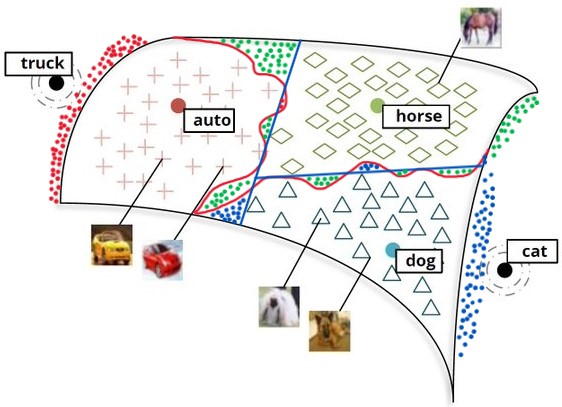
\includegraphics[width=1\textwidth, height=1\textheight, keepaspectratio]{manifold-hyp}
    \end{minipage}
    \begin{minipage}[c]{0.49\textwidth}
        \vspace{0pt}
        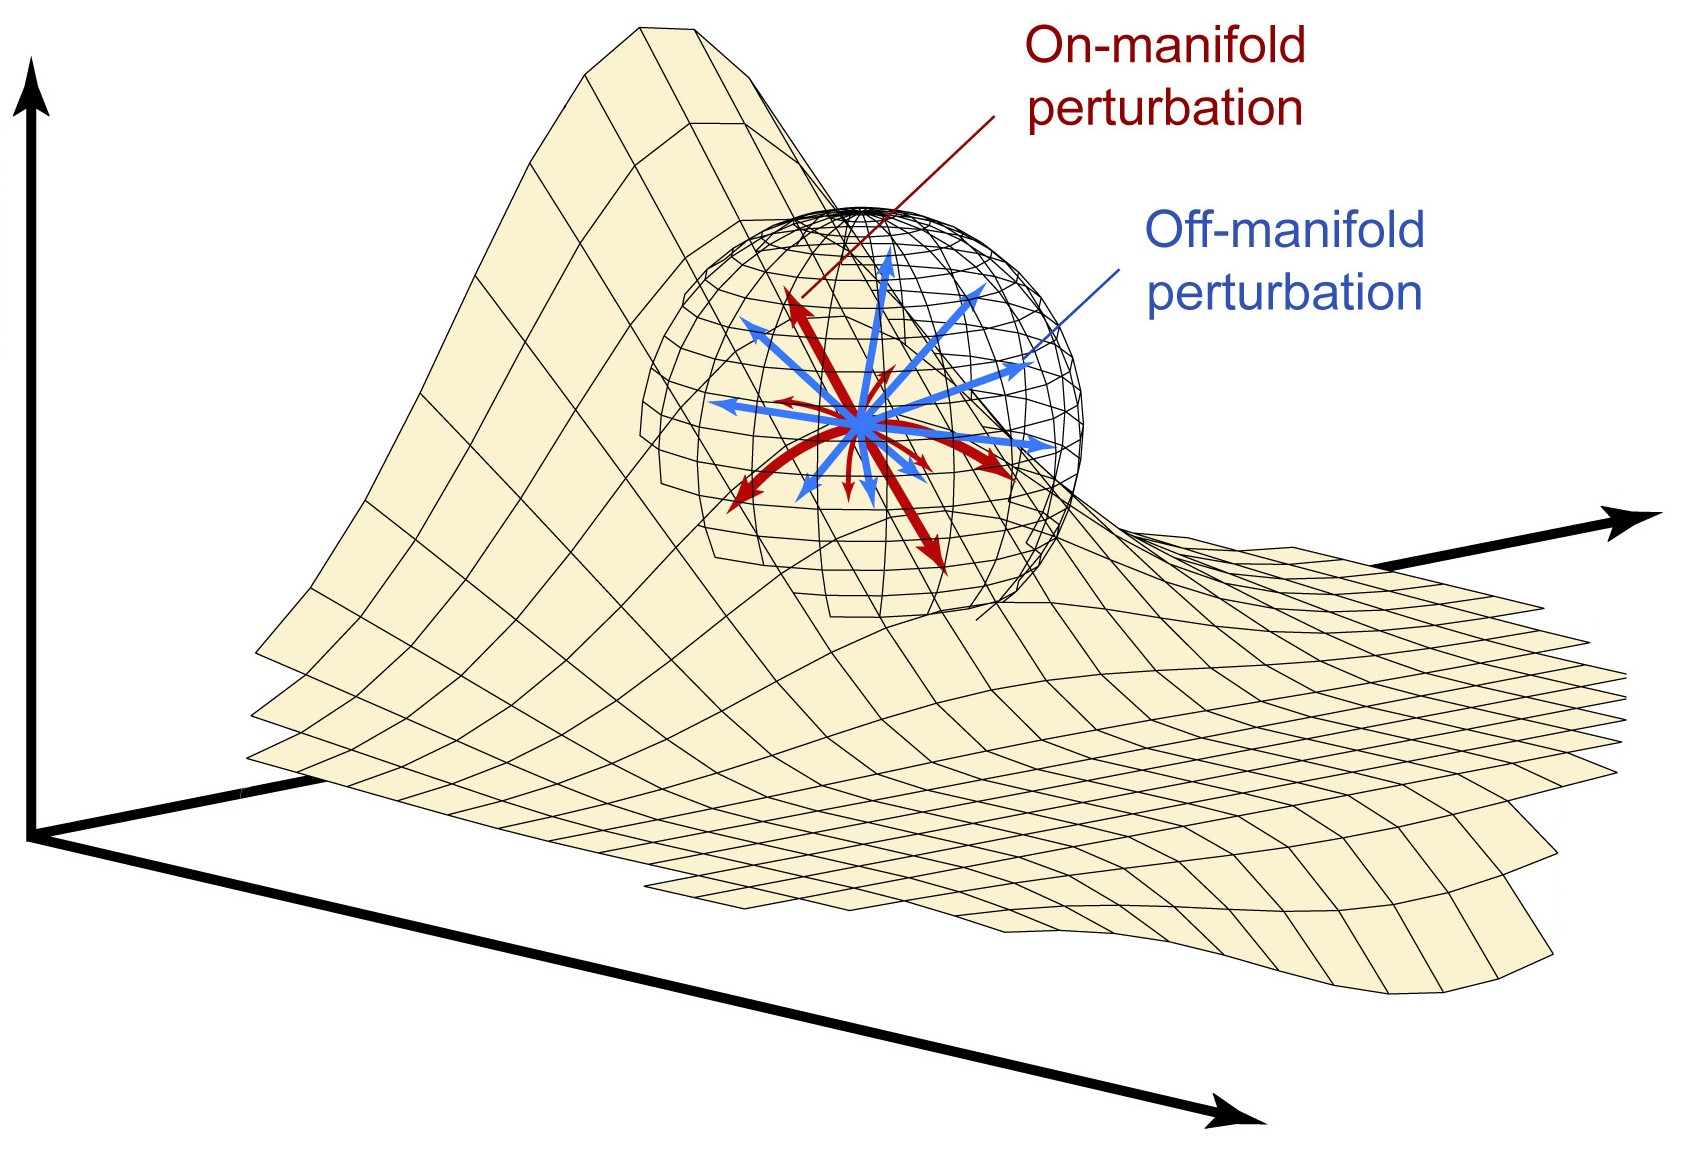
\includegraphics[width=1\textwidth, height=1\textheight, keepaspectratio]{manifold_ball_perturbations}
    \end{minipage}
    \hfill\break

    \texttt{CARSO} acts mainly as an \textit{on manifold re-projector}!

    \end{frame}

    \begin{frame}{\protect{\emoji{speaking-head}} Discussion (III)}

        \begin{block}{Time: a hidden cost?}
            Regardless of model performance, the \textit{training time} required for the \texttt{CARSO} portion of the alone is $\sim$ equivalent to that of \texttt{IAT} for the classifier. This results in a twofold increase in training time.

            Inference time sees a $\sim1500$-fold increase.
        \end{block}

    \underline{Note, however, that...}
    \begin{itemize}
        \item Overall training time is still (\textit{much}, even \textit{very much}; see \texttt{DefenseGAN} \textit{e.g.}) shorter than most \textit{better-than-\texttt{IAT}} approaches!
        \item \textit{W.r.t.} inference time, the method was originally targeted at \textit{high-stakes}, scenarios where such trade-off is acceptable. In case of realtime scenarios, also thanks to increased robustness, one can resort to \textit{stream thinning} (or \textit{fast-vs-slow} systems) if \texttt{CARSO} is deemed important.
    \end{itemize}
    \end{frame}

}


    % !TeX spellcheck = en_GB

\section{\protect{\emoji{rocket}} Conclusion and future outlook}{

    \begin{frame}{\protect{\emoji{rocket}} Where did we came from, where do we go?}

        We talked about \texttt{CARSO} -- a novel framework devised to foil \textit{gradient-based adversarial attacks}, specifically targeted at image classification -- showing noteworthy improvements upon \texttt{IAT}, a strong contribution to \textit{off-manifold-to-on-manifold reprojection}, and solid \textit{innate robustness}.

        Experimental scope can be broadened, though:
        \begin{itemize}
            \item Proper, meticulous hyperparameter tuning;
            \item Different architectures;
            \item More complex datasets;
            \item Different \textit{media} (text, sequences, \etc\dots);
            \item Broader attack \textit{coverage} (e.g. against \textit{adaptive attacks});
            \item Comparison with additional defences.
        \end{itemize}

    \end{frame}

    \begin{frame}{\protect{\emoji{rocket}} Through \texttt{CARSO}, beyond \texttt{CARSO}}

        The work required to develop and assess \texttt{CARSO} evoked suggestions reaching far longer and broader than expected. Chiefly, in order of increasing conceptual distance...

        \begin{itemize}
            \item The idea that \textit{adaptive} defences may exist, explicitly steering their behaviour on the basis of the geometric properties of inputs or attacks faced. \texttt{CARSO} might even one (though embryonic, immature) of this kind.
            \item Weight-agnostic layers operating at the \textit{feature-specific} (or, traditionally, \textit{architecture/dataset-specific}) level -- able to produce \textit{zero-gradient} in expectation, without masking it.
            \item The possibility of informing the development (or... the \textit{training}?!) of \textit{deep learning} architectures with (the information contained in) neural activity recordings -- for the sake of one or the other, or both. And, why not: \textit{live-subject} recordings! \protect{\emoji{mouse}}
        \end{itemize}
    \end{frame}

    \begin{frame}{\protect{\emoji{rocket}} Hopefully part of a \textit{broader} endeavour... (I)}
        \centering
        \vspace*{10px}
        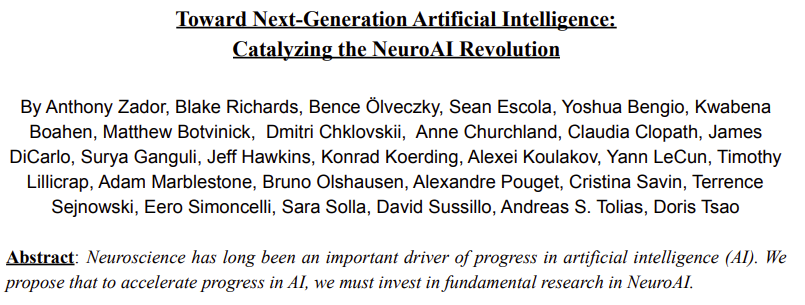
\includegraphics[width=0.98\textwidth, height=0.7\textheight, keepaspectratio]{towards_neuro_ai_paper_heading.png}
        \vspace*{10px}

        (Zador et al., 2022 -- \textit{ArXiv, abs/2210.08340})
        \vspace*{10px}
    \end{frame}

    \begin{frame}{\protect{\emoji{rocket}} Hopefully part of a \textit{broader} endeavour... (II)}
    \centering
    \vspace*{10px}
    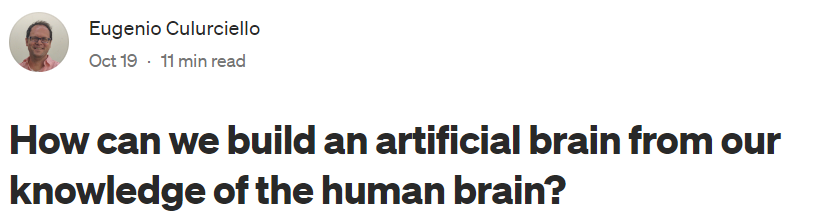
\includegraphics[width=0.98\textwidth, height=0.7\textheight, keepaspectratio]{culurciello_medium.png}
    \vspace*{10px}

    (Eugenio Culurciello, 2022 -- \textit{Medium.com}, see: {https://cutt.ly/culurciello\_brain\_2022})
    \vspace*{10px}
\end{frame}
}

    % !TeX spellcheck = en_GB
\phantomsection
\begin{frame}{Thanks for your attention!}
    \centering
    \vspace*{15px}
    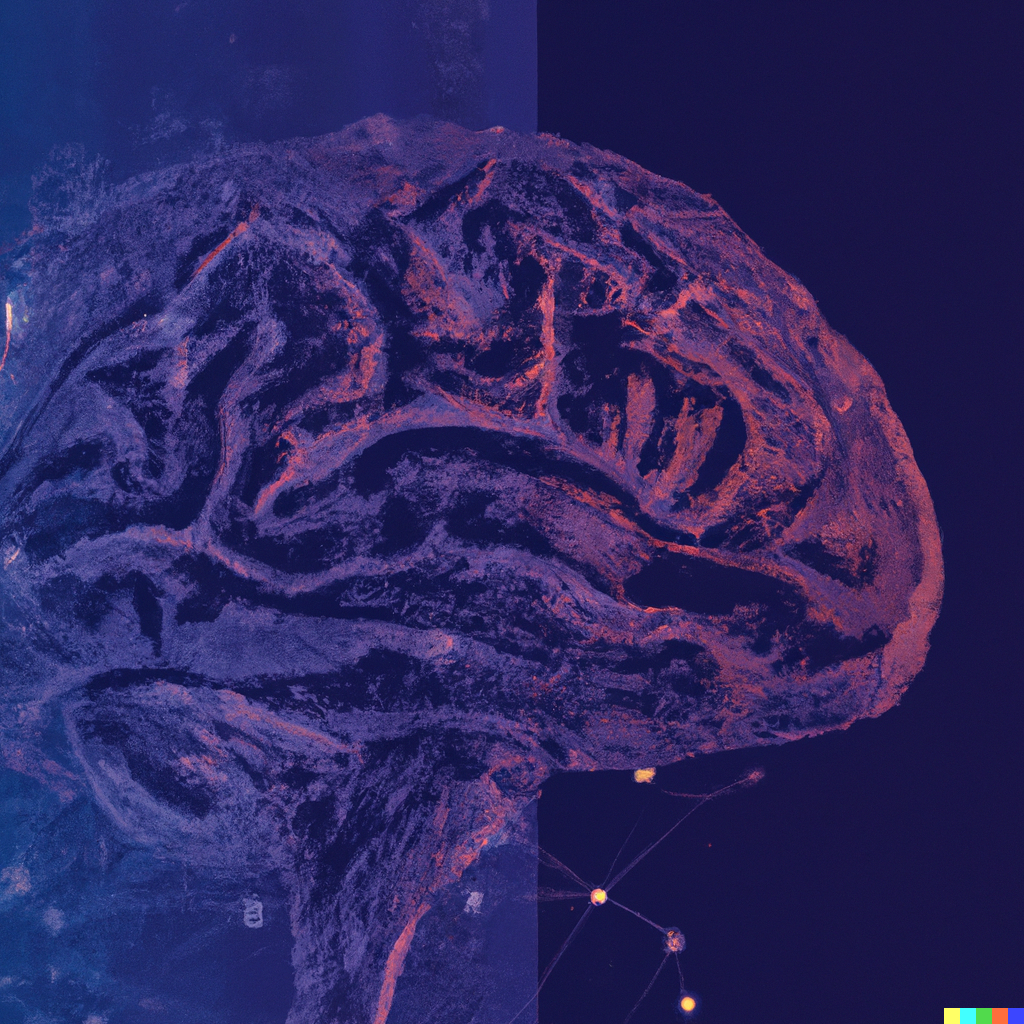
\includegraphics[width=0.7\textwidth, height=0.7\textheight, keepaspectratio]{dallecarso}
    \vspace*{10px}

    \texttt{[ \href{https://ballarin.cc/carsocode}{https://ballarin.cc/carsocode} ]}
\end{frame}
\end{document}
